\documentclass{article}
\usepackage{authblk}
\usepackage{acro}
\usepackage{amsmath}
\usepackage{amsfonts}
\usepackage{caption}
\usepackage{ccaption}
\usepackage[margin=20truemm]{geometry}
\usepackage[dvipdfmx]{graphicx}
\usepackage{hyperref}
\usepackage{url}

\title{\empty}
\author{\empty}
\date{\empty}

\DeclareCaptionLabelFormat{supplemental}{\textbf{Figure S#2}}
\captionsetup[figure]{labelformat=supplemental}

\urlstyle{same}

\begin{document}
\pagenumbering{roman}
\maketitle

\section*{Appendices}
\subsection*{Supplemental Information}
\subsubsection*{Cell clusters vs cells classes}
A cell cluster refers to a stochastic chunk of samples neighbouring each other in the data space or spacific feature 
space designed via the data analysis. Hence, cell clusters can be defined without introducing GRNs or eigen-cascades. 
Contrary, a cell class refers a set of samples, which can be treated identical, and their biological features 
characterized with the eigen-cascades. In this context, what is identical can be defined by a clustring function (i.e., 
a mapping between samples and the clusters that they belong to) of choice. Therefore, the term cell class 
emphasizes the randomness of a cell cluster and always tagged with the concept of eigen-cascades. On the other hand, 
we use cell cluster to refer some data-driven groups of cells in a more neutral nuance.

\subsubsection*{
  The vertex set $V_{[x]}(G)$, the edge set $E_{[x]}(G)$, and the eigen-cascades $C_{[x]}(G)$ of a cell class $[x]$
}
A graph $(V, E)$ is a pair of the vertex set $V$ and the edge set $E$. To create a graph of a 
set of genes $G$ based on the statistical dependencies of the genes, the vertex set $V(G)$ and the 
edgeset $E(G)$ are introduced as follows:
\begin{equation}\label{V}
  V(G):=G \stepcounter{equation} \tag{S-\theequation}
\end{equation}
\begin{equation}\label{E}
  E(G):=\{(g_1, g_2)\;|\;g_1,g_2\in G\; s.t. \;g_1\neq g_2\;\text{and}\; g_1\;\text{is dependent on}\;g_2\}.
  \stepcounter{equation} \tag{S-\theequation}
\end{equation}
It is important to note that $(V(G),E(G))$ itself refers to a multigraph and we need to equate $(g_1,g_2)$ 
and $(g_2,g_1)$ to create GRNs (undirected simple graphs). In the previous article, we introduced 
asymmetrical notations for edge sets to build up our theory from causal networks and relaxed 
the restriction by replacing the causalities with the statistical dependencies. In this section, 
we adopted the same style for consistency even though the statistical dependency of two variables is symmetrical.

We also introduced a notation $\{g_1, g_2\}_{g_1}$ where $^\forall g_1,g_2\in G$ such that $g_1$ is dependent on $g_2$, representing an 
indexed set with the index $g_1\in\{g_1, g_2\}$ (note that the symmetry of statistical dependency induces symmetry 
$\{g_1, g_2\}_{g_1}=\{g_1, g_2\}_{g_2}$). We named such index sets cascades. The inclusion of $g_1$ being dependent on itself leads to 
the expression $\{g_1, g_1\}_{g_1}$; however, mathematical set rules simplify this to $\{g_1\}_{g_1}$. Notably, these singleton sets are 
also considered valid representations of cascades. The eigen-cascades of a cell class $[x]$ are the cascades that can be 
inferred from $[x]$, which is the cell class that a sample $x$ belongs. As all cascades are either singletons or sets of two 
elements, the set of the eigen-cascades $C_{[x]}(G)$ of $[x]$ equals to the union of $V_{[x]}(G)$ and $E_{[x]}(G)$ defined as follows:
\begin{equation}\label{Vx}
  V_{[x]}(G):=\{c|c\in C_{[x]}(G)\; s.t.\; |c|=1\}=\{\{g\}_g|g\in G\}
  \stepcounter{equation} \tag{S-\theequation}
\end{equation}
\begin{equation}\label{Ex}
  E_{[x]}(G):=\{c|c\in C_{[x]}(G)\; s.t.\; |c|=2\}=C_{[x]}(G)\setminus V_{[x]}(G).
  \stepcounter{equation} \tag{S-\theequation}
\end{equation}

Juxtaposing the given definitions from Eq. \eqref{V} to Eq. \eqref{Ex}, $V_{[x]}(G)$ and $V_x(G)$ 
as well as $E_{[x]}(G)$ and $E_x(G)$ have similar formulations. More precisely, $V_{[x]}(G)$ is isomorphic to $G$ and 
$E_{[x]}(G)$ can be isomorhic to some edge set (e.g., a map $\varphi:\{g_1,g_2\}_{g_1}\mapsto(g_1,g_2)$ 
is an isomorphism and $\varphi(E_{[x]}(G))$ is a valid edge set). Accordingly, a graph $(G, \varphi(E_{[x]}(G)))$ can be formed 
referring the eigen-cascades, and the pair of $C_{[x]}(G)$ and $(G, \varphi(E_{[x]}(G)))$ show one-to-one correspondence.
Concisely, $V_{[x]}(G)$ and $E_{[x]}(G)$ can be regarded as the vertex set and the edge set.

It is important to note that the mathematical discussions to extend the notion of cascades to eigen-cascades of 
cell classes include various notations, operations, and hypotheses that can sound confusing or untrivial. 
In this article, we simply introduced the notations of $[x]$ and $C_{[x]}(G)$ aiming to shortcut the redundant part. 
We recommend to refer to the original article for readers interested in the detailed explanations.

\subsubsection*{
  The logistic model of DOR
}
Although the mean expression values and the DOR values show a non-linear relationship, we tried to find a simple 
non-linear conversion that enables the mean expression values to linearly fit to the DOR values. We leveraged the 
logistic transformation (i.e., inverse logit transformation) so that the transformed values becomes positive and less 
than 1. Introducing $u$ to be the variable for the transformed values as follows, we tried to fit the parameter $b$ ($b>0$) 
so that $DOR\sim -2u + 2$ by minimizing the MSE:
\begin{equation}\label{logistic transformation}
  u := \frac{1}{1+e^{-b\cdot Mean}}.
  \stepcounter{equation} \tag{S-\theequation}
\end{equation}
Note that the minimal value of $u$ is 0.5 (when $Mean=0$) and the following equation holds for the limit:

\begin{equation}\label{lim}
  \lim_{Mean\rightarrow\infty}u=1
  \stepcounter{equation} \tag{S-\theequation}.
\end{equation}
In addition to those properties, the range of DOR is $0\leq DOR\leq 1$, and they are the reasons why we designed the 
fitting line as $DOR\sim -2u + 2$. Consequently, the final form of the fitting curve can be denoted as follows:
\begin{equation}\label{logistic model}
  DOR\sim -\frac{2}{1+e^{-b\cdot Mean}}+2.
  \stepcounter{equation} \tag{S-\theequation}
\end{equation}

\subsubsection*{Inverse predictions of LM, Poisson regression, and NB regression}
The inverse prediction of LM can be formulated as follows by solving Eq. \eqref{logistic model} iff $DOR\neq 0$:
\begin{equation}\label{inverse lm}
  Mean\sim\log{(\frac{2-DOR}{DOR})^\frac{1}{b}}.
  \stepcounter{equation} \tag{S-\theequation}
\end{equation}

As we used the logarithmic link function for both the Poisson regression models and the NB regression models, 
those models can be formulated as follows:
\begin{equation}\label{glm}
  DOR\sim e^{b_0+b_1\cdot Mean}.
  \stepcounter{equation} \tag{S-\theequation}
\end{equation}
Therefore, the inverse predictions of those models can be formulated as follows by solving Eq. \eqref{glm} iff $DOR\neq 0$:
\begin{equation}\label{inverse glm}
  Mean\sim\frac{-b_0+\log{DOR}}{b_1}.
  \stepcounter{equation} \tag{S-\theequation}
\end{equation}

It is noteworthy that the $Mean$ value diverges into infinity as $DOR$ approaches to zero regardless of the choice 
of the models. Therefore, performance comparison of the inverse prediction models was performed while excluding the data 
with zero $DOR$ values to avoid metrics such as MAE diverge into infinity (in which case the result indicates 
that all models perform exactly as poorly as the others by generating infinity prediction errors on average).

\subsubsection*{Benchmarking DOR regression models with Mereu2020 datasets}
For benchmarking DOR regression models (namely LM, Poisson regression model, and NB regression model), we 
used Mereu2020 dataset families so that we can evaluate the performance of those models when the data were 
acquired in various sequencing protocols. Likewise we did on PBMC3k dataset, we made LMs, Poisson regression 
models, and NB regression models for respective datasets (\figurename{ S7A-O}). Then we measured MSE (\figurename{ S8B}), 
MAE (\figurename{ S8C}), MAE of the inverse-prediction models (\figurename{ S8D}), and MaxAE of the inverse-prediction 
models (\figurename{ S8E}) to evaluate their performance.

Unlike the result from PBMC3k dataset, LM underperformed Possion and NB regression models in most cases 
(except for Chromium V2 (sn), Chromium V3, C1HT-medium, and C1HT-small) in terms of MSE (\figurename{ S8B}). 
Similar results were reproduced in terms of MAE even though all models scored quite small MAE values (\figurename{ S8C}).
Although LM slightly underperformed the two conventional regression models in explaining the relationship 
between mean expressions and DOR values in general cases, LM showed stable performance in the inverse-prediction 
tasks scoring less than 0.1 MAE in all cases (\figurename{ S8D}), and even outperformed Poisson and NB regression models 
in terms of MaxAE (\figurename{ S8E}) suggesting that LM performed better than the other two models at low DOR 
values. Those results indicated that LM models work as calibration curves that can transform DOR and mean 
expression values interchangeably in wide ranges of those input values, while the conventional regression models 
have more weights on domains where samples densely distribute (regularly high-DOR and low-mean-expression 
areas) to outperform LM in terms of MSE, MAE, and MAE of the inverse prediction in general.

\subsubsection*{
  The preimage and general scRNA-seq data transformation
}
Let $^\forall A,B,C$ be sets such that $C\subset B$, and let $f:A\rightarrow B$ be a map. 
The preimage of $C$ under $f$ (denoted as $f^{-1}[C]$) is defined as follows:
\begin{equation}\label{preimage}
  f^{-1}[C]:=\{a\;|\;a\in A\;s.t.\;f(a)\in C\}.
  \stepcounter{equation} \tag{S-\theequation}
\end{equation}
Therefore, a function $\psi: \mathbb{N}\rightarrow\mathbb{R}$ such that $\psi^{-1}[\{0\}]=\{0\}$ returns zero 
if and only if the input value is zero. This property is essential for $Coverage_{[x]}$ to identify non-zero values.

Let $\psi_R:\mathbb{N}\rightarrow \mathbb{Q}$ as the RPM transformation from the raw counts, and let $\psi_L:\mathbb{Q}\rightarrow \mathbb{R}$ be the transformation 
from RPM values to $\log_k(RPM+1)$ for all $k>0$. It is trivial that $\psi_R^{-1}[\{0\}]=\{0\}$ and $\psi_L^{-1}[\{0\}]=\{0\}$ hold.
Accordingly, the conversion from raw counts to $\log_k(RPM+1)$ values are $\psi_L\circ\psi_R$, and the following equation holds:
\begin{equation}\label{raw2logrpm}
  (\psi_L\circ\psi_R)^{-1}[\{0\}]=\psi_R^{-1}[\psi_L^{-1}[\{0\}]]=\psi_R^{-1}[\{0\}]=\{0\}.
  \stepcounter{equation} \tag{S-\theequation}
\end{equation}

\subsubsection*{
  An example where WHQPM is undefined
}
Taking look at the definition of $Whqpm$, it is clear that the formula holds iff $|E_{[x]}(G)|+\sum_{g\in G}Coverage_{[x]}(g)\neq 0$. 
Given that both $|E_{[x]}(G)|$ and $\sum_{g\in G}Coverage_{[x]}(g)$ are non-negative, $Whqpm$ decomes undifined when those two 
terms are both zero. Such condition is readily satisfied when the GRN of the subjective cell class $[x]$ is characterized 
with genes completely absent in $[x]$ exhibiting zero coverages (i.e., DOR values of those genes are all 1). In such 
case, not only $\sum_{g\in G}Coverage_{[x]}(g)=0$ but also $|E_{[x]}(G)|$ becomes 0 (otherwise $^\forall e\in|E_{[x]}(G)$ is undefined). The status 
of $|E_{[x]}(G)|$ varies depending on the choice of GRN formation algorithm, in other words, computational methods to 
assign edges among vertexes. While the correlation-based method and the chi-squared test-based method coupled 
with the dropout-based binarization are not applicable for the case where the mean expression values are all zero 
and all samples in $[x]$ are negative for all genes. Alternatively, Fisher's exact test is an available option for the 
algorithm to compute the edges, but the null hypotheses fail to be rejected in those setting resulting in $|E_{[x]}(G)|=0$.

Consequently, $Whqpm$ is undefined when the GRN of $[x]$ is formed with genes such that $\sum_{g\in G}Coverage_{[x]}(g)=0$. 
By design, WHQPM prevents ill-defined characterization of the similarity between two cell classes by staying 
undefined when the subjective cell class is represented exclusively with uncharacteristic genes.

\newpage
\subsection*{Supplemental Figures}
\begin{figure}[htb]
  \centering
  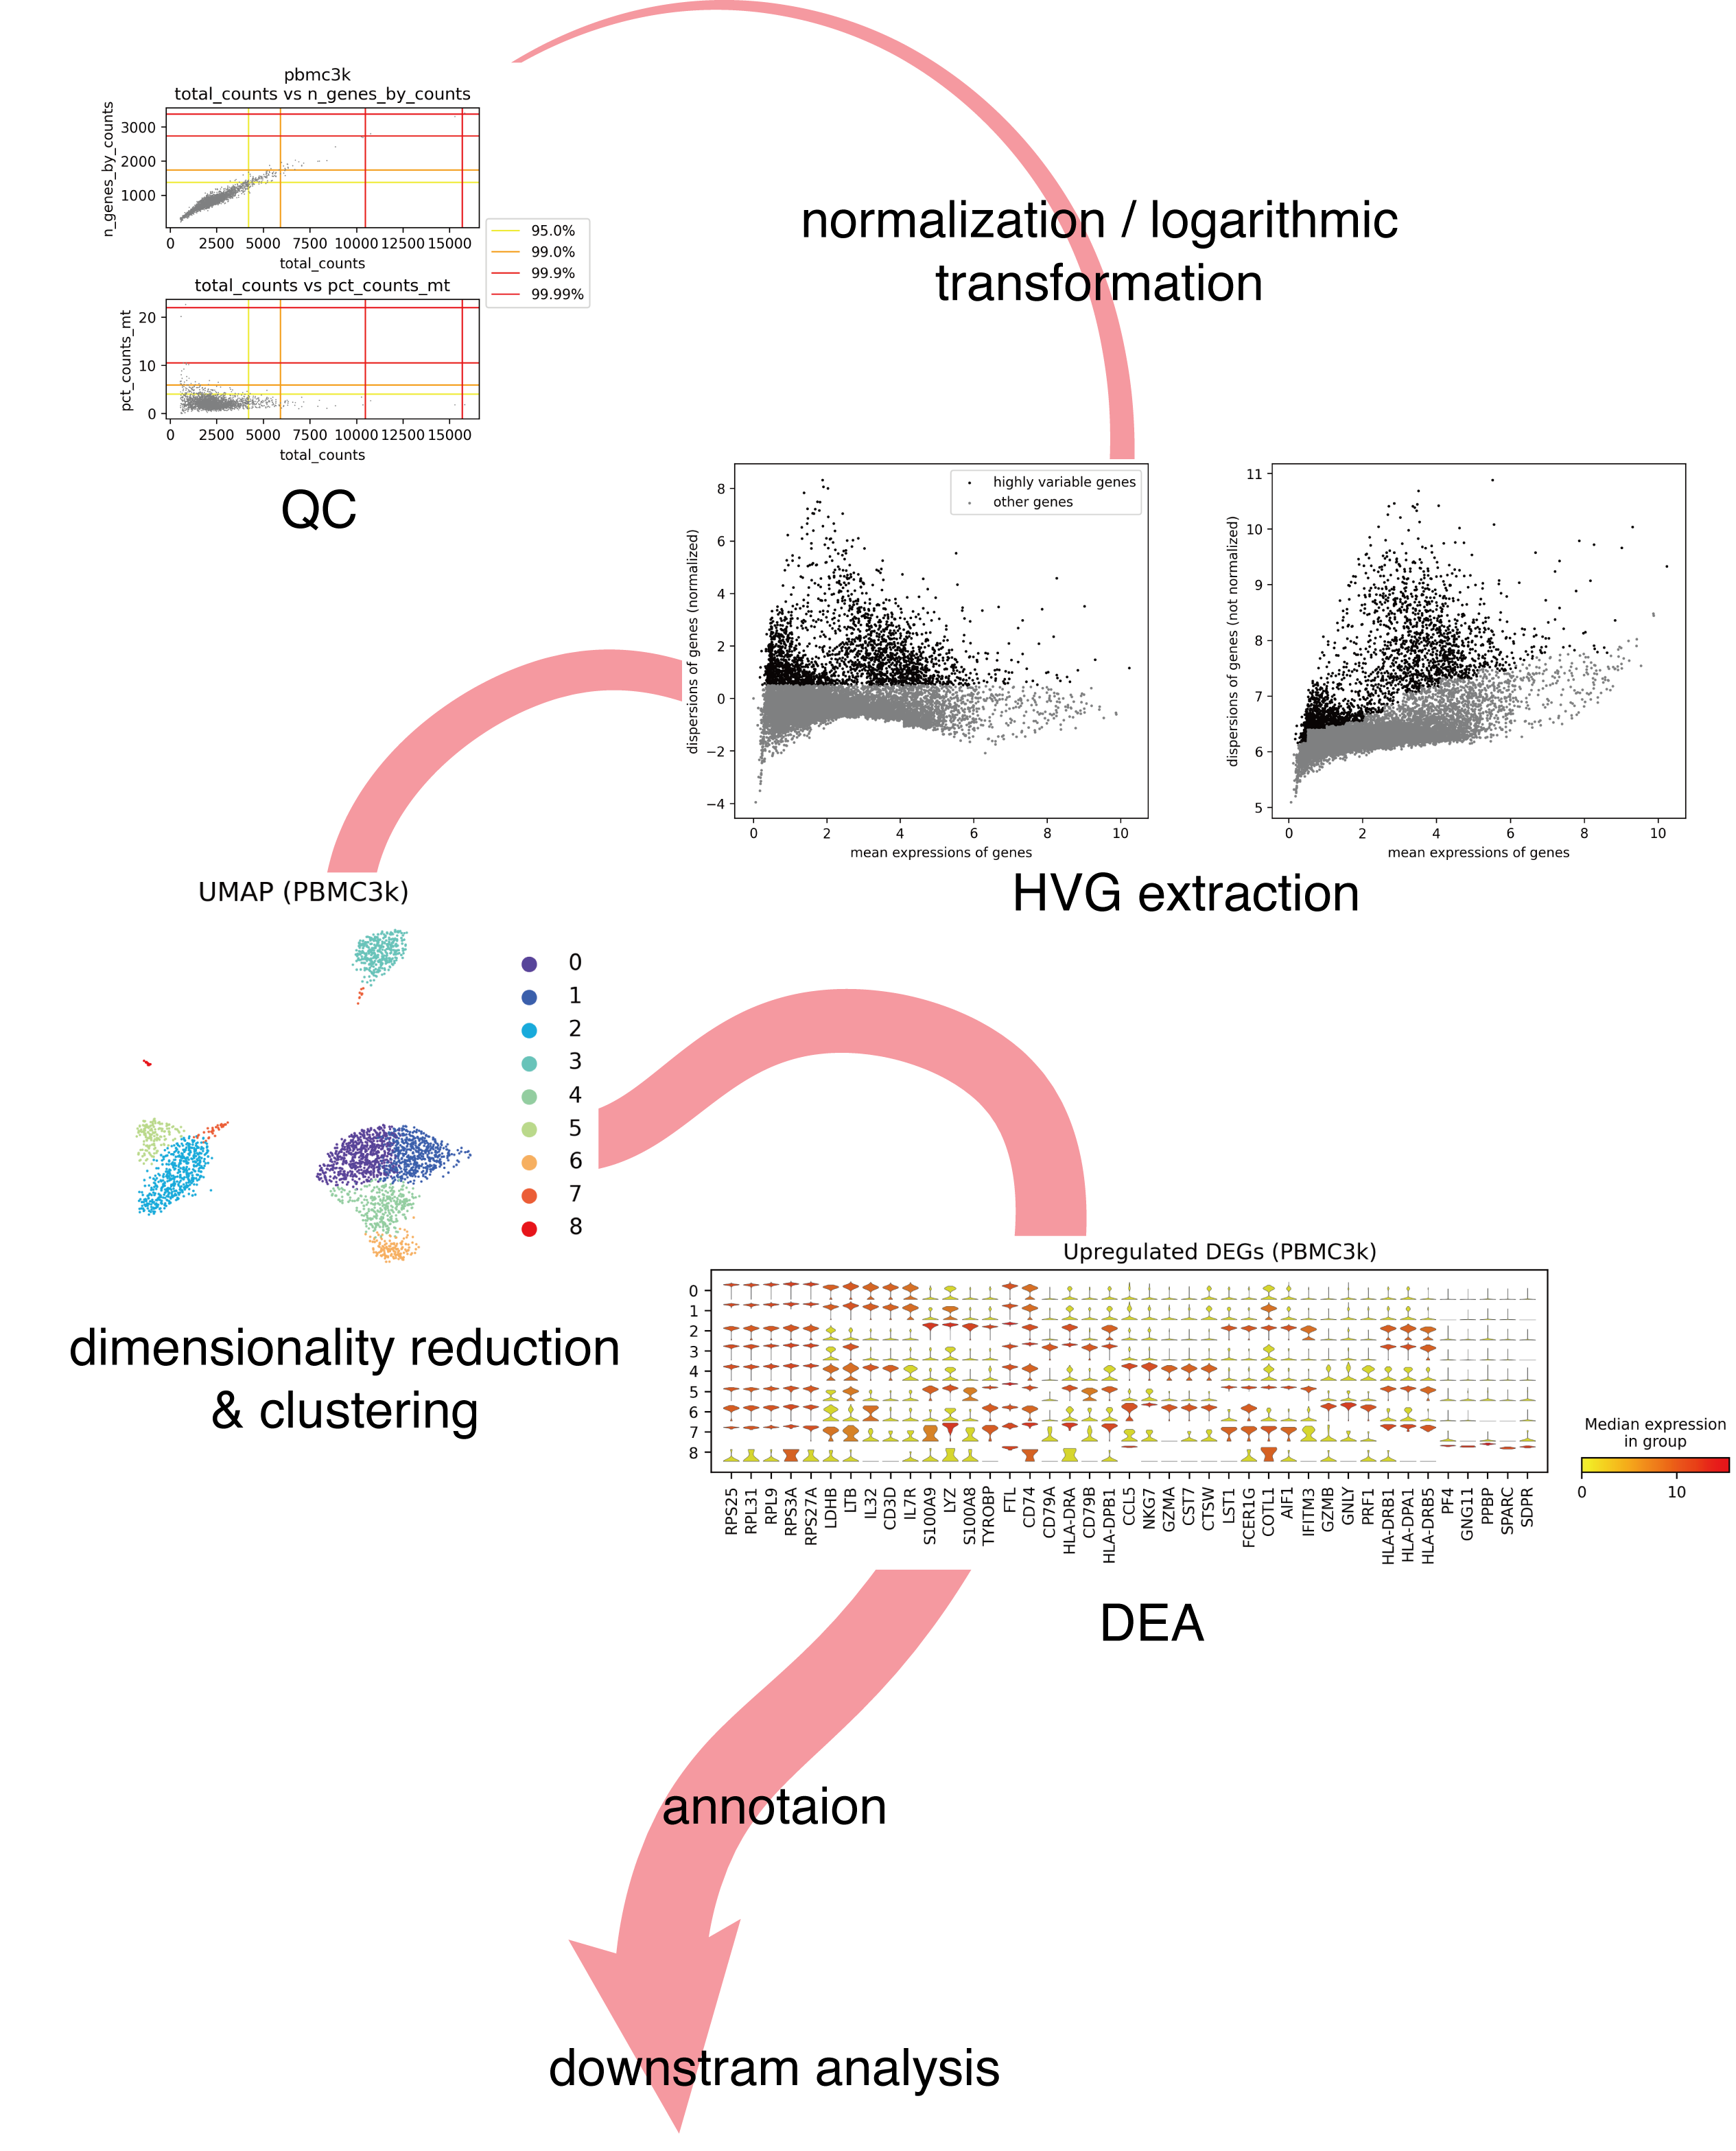
\includegraphics[scale=0.6]{./figs/exported/figure_s1.png}
  \caption{Standard workflow of scRNA-seq analysis}
  \legend{
    A scheme that shows a standard process of scRNA-seq data analysis. 
    The plots were generated during the analysis of PBMC3k.
  }
  \label{fig_s1}
\end{figure}
\begin{figure}[htb]
  \centering
  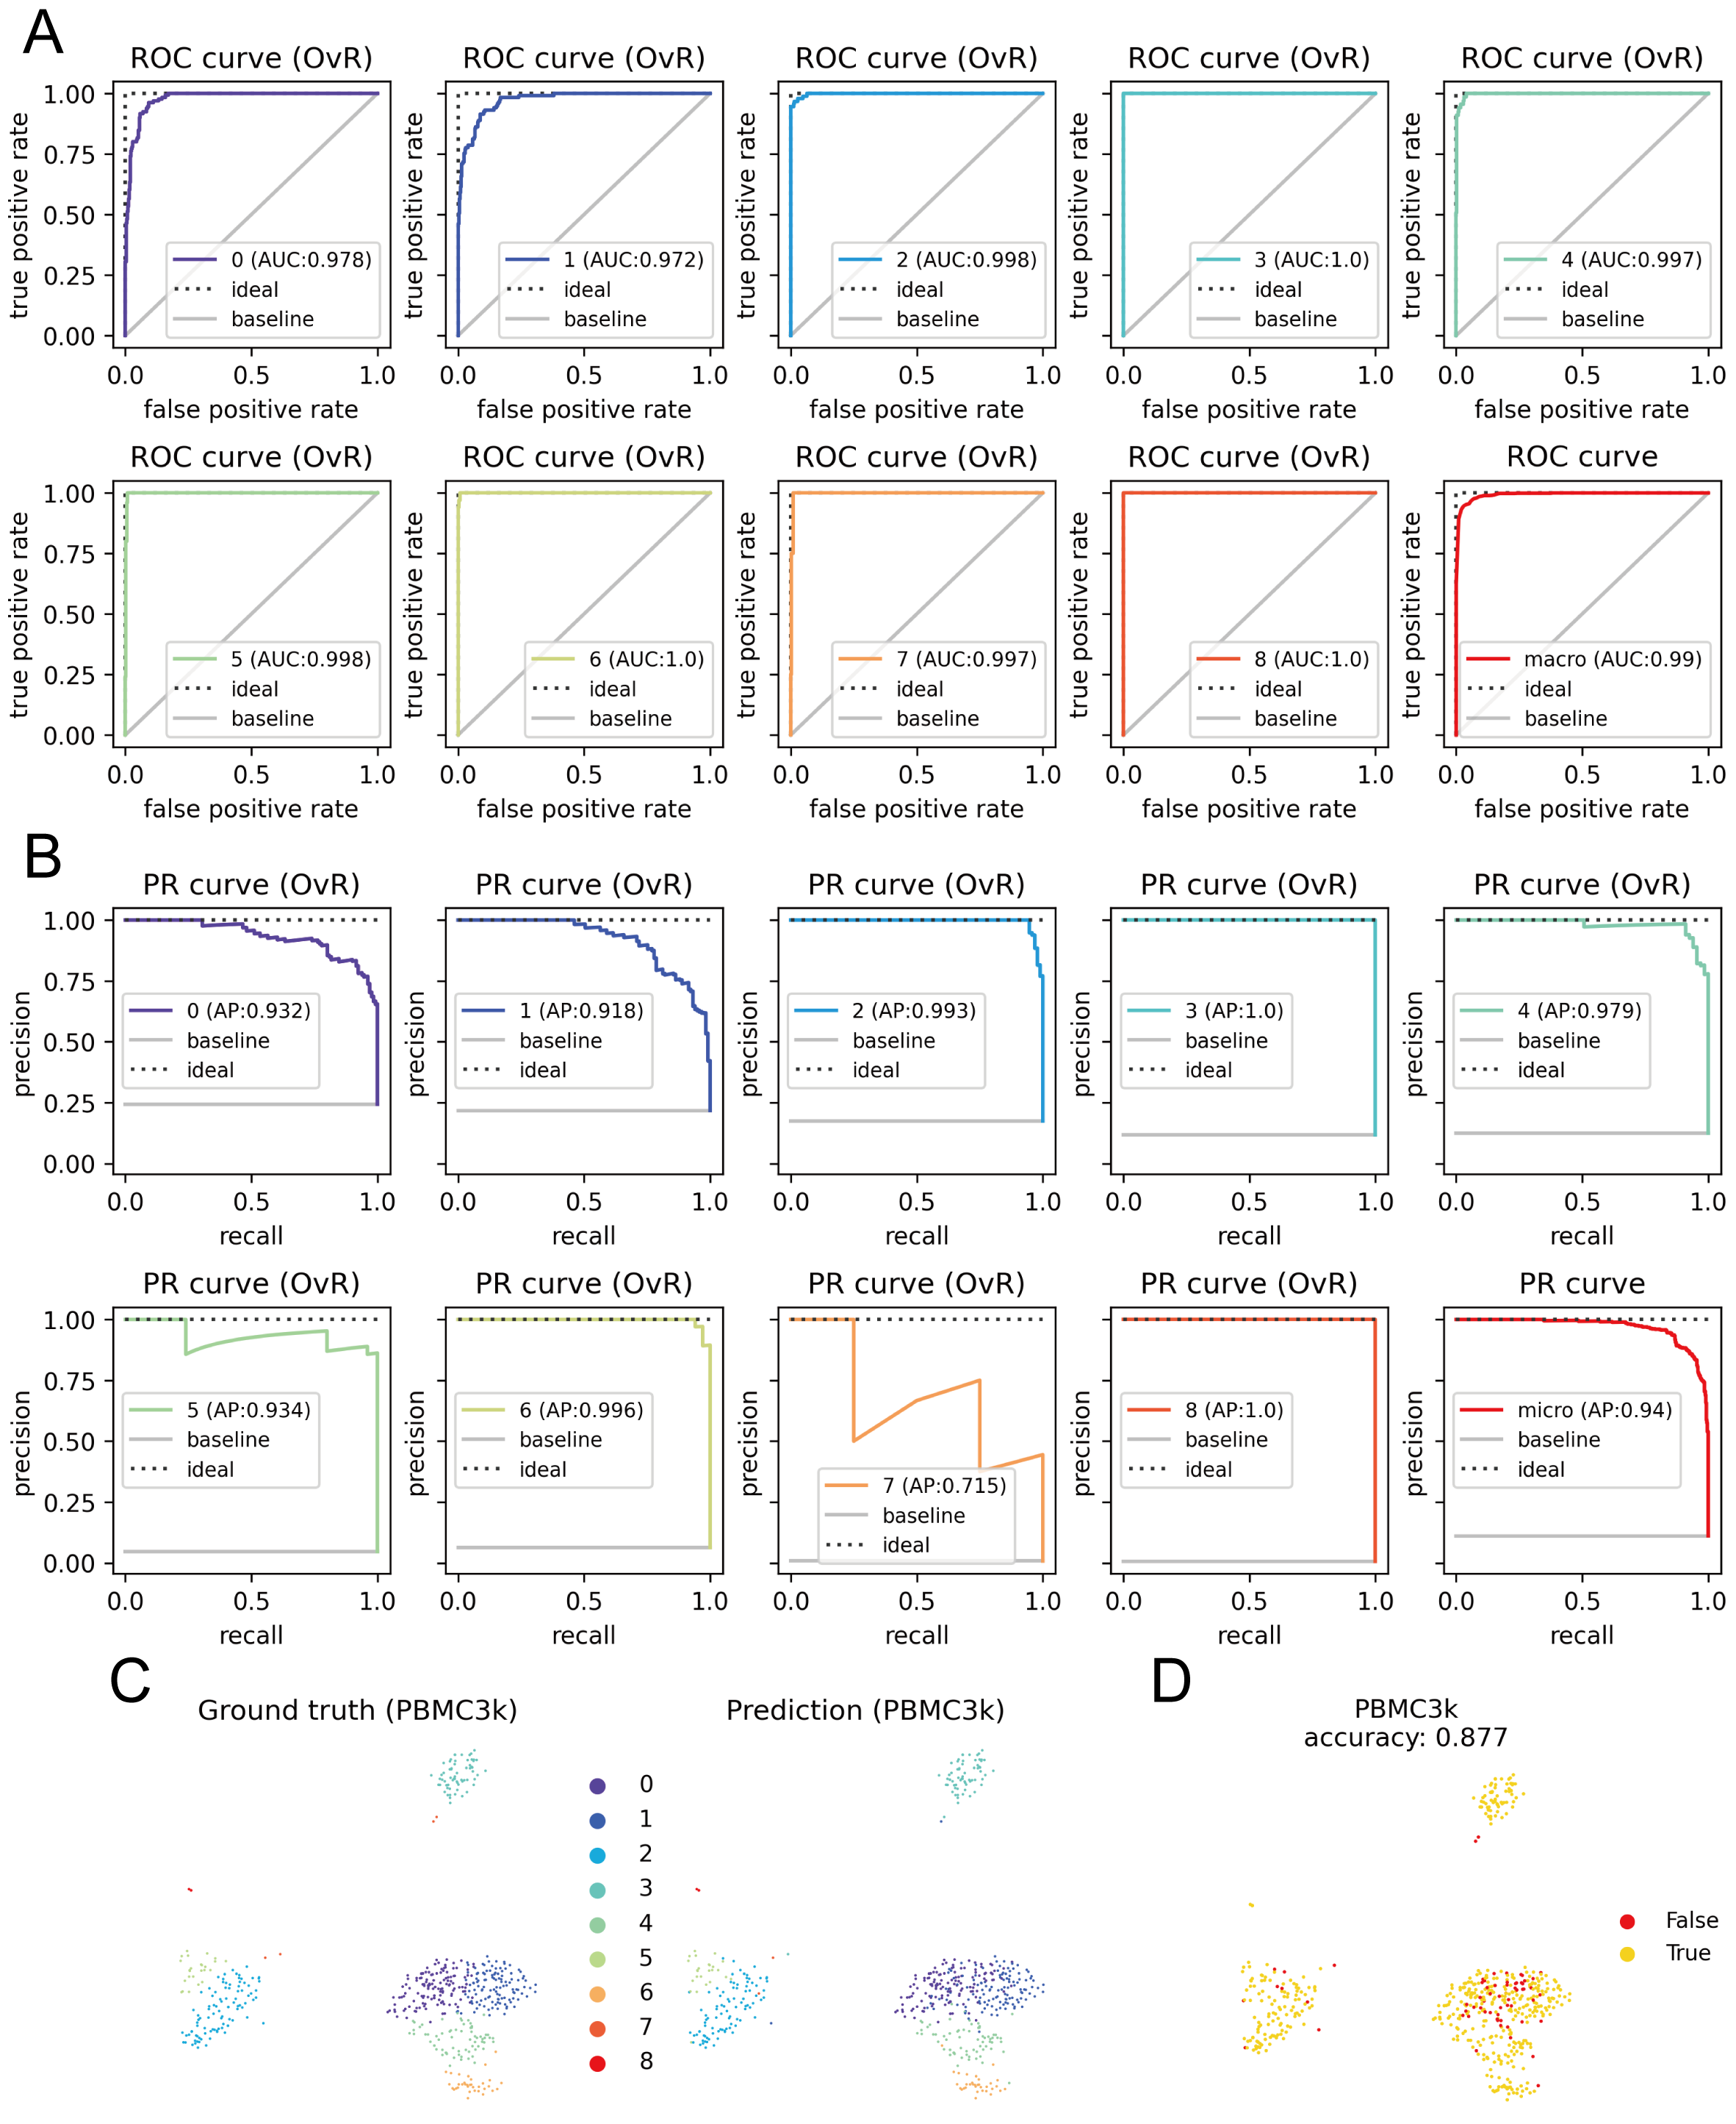
\includegraphics[scale=0.7]{./figs/exported/figure_s2.png}
  \caption{The performance of the GBDT model}
  \legend{
    \textbf{A}: The OvR ROC curves of the clusters 0$\sim$8 and their macro average
    \textbf{B}: The OvR PR curves of the clusters 0$\sim$8 and their micro average
    \textbf{C}: A pariwise comparison of the ground-true labels and the predictions
    \textbf{D}: A UMAP visualization of the prediction accuracy
  }
  \label{fig_s2}
\end{figure}
\begin{figure}[htb]
  \centering
  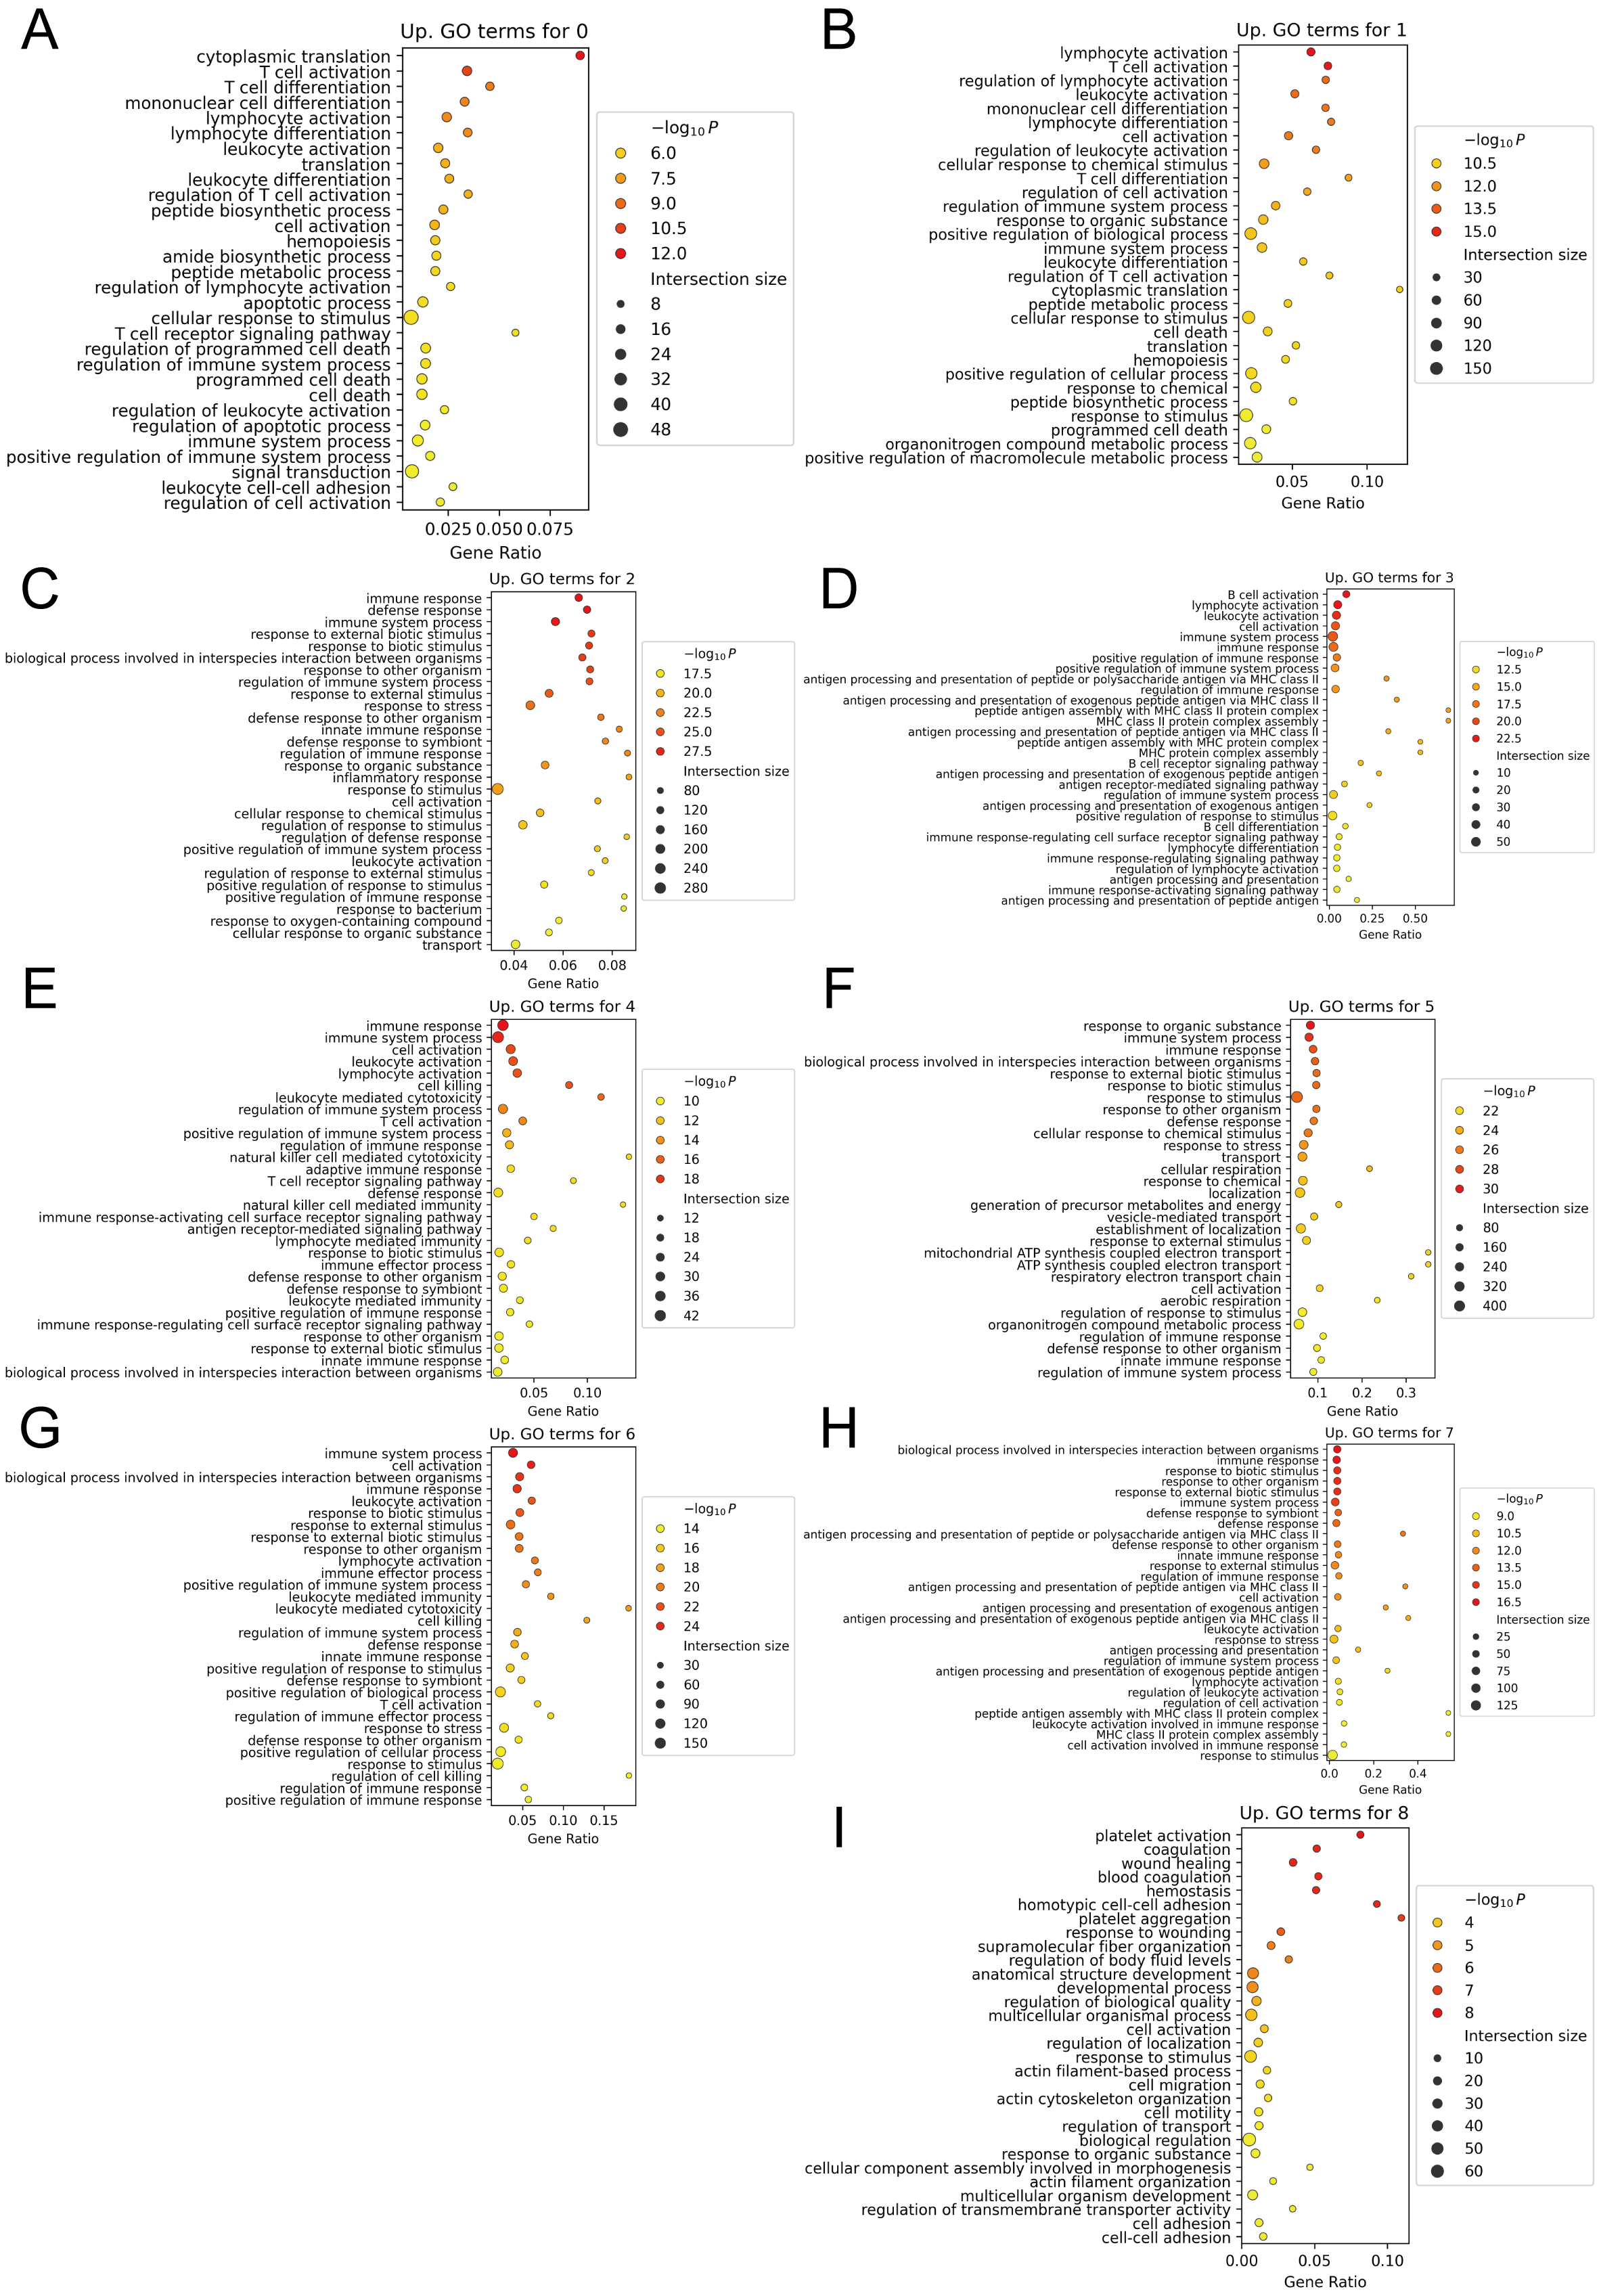
\includegraphics[scale=0.7]{./figs/exported/figure_s3.png}
  \caption{The top 10 features of the clusters in PBMC3k}
  \legend{
    \textbf{A-I}: The top 10 features (based on SHAP values) for cluster 0$\sim$8 respectively
  }
  \label{fig_s3}
\end{figure}
\begin{figure}[htb]
  \centering
  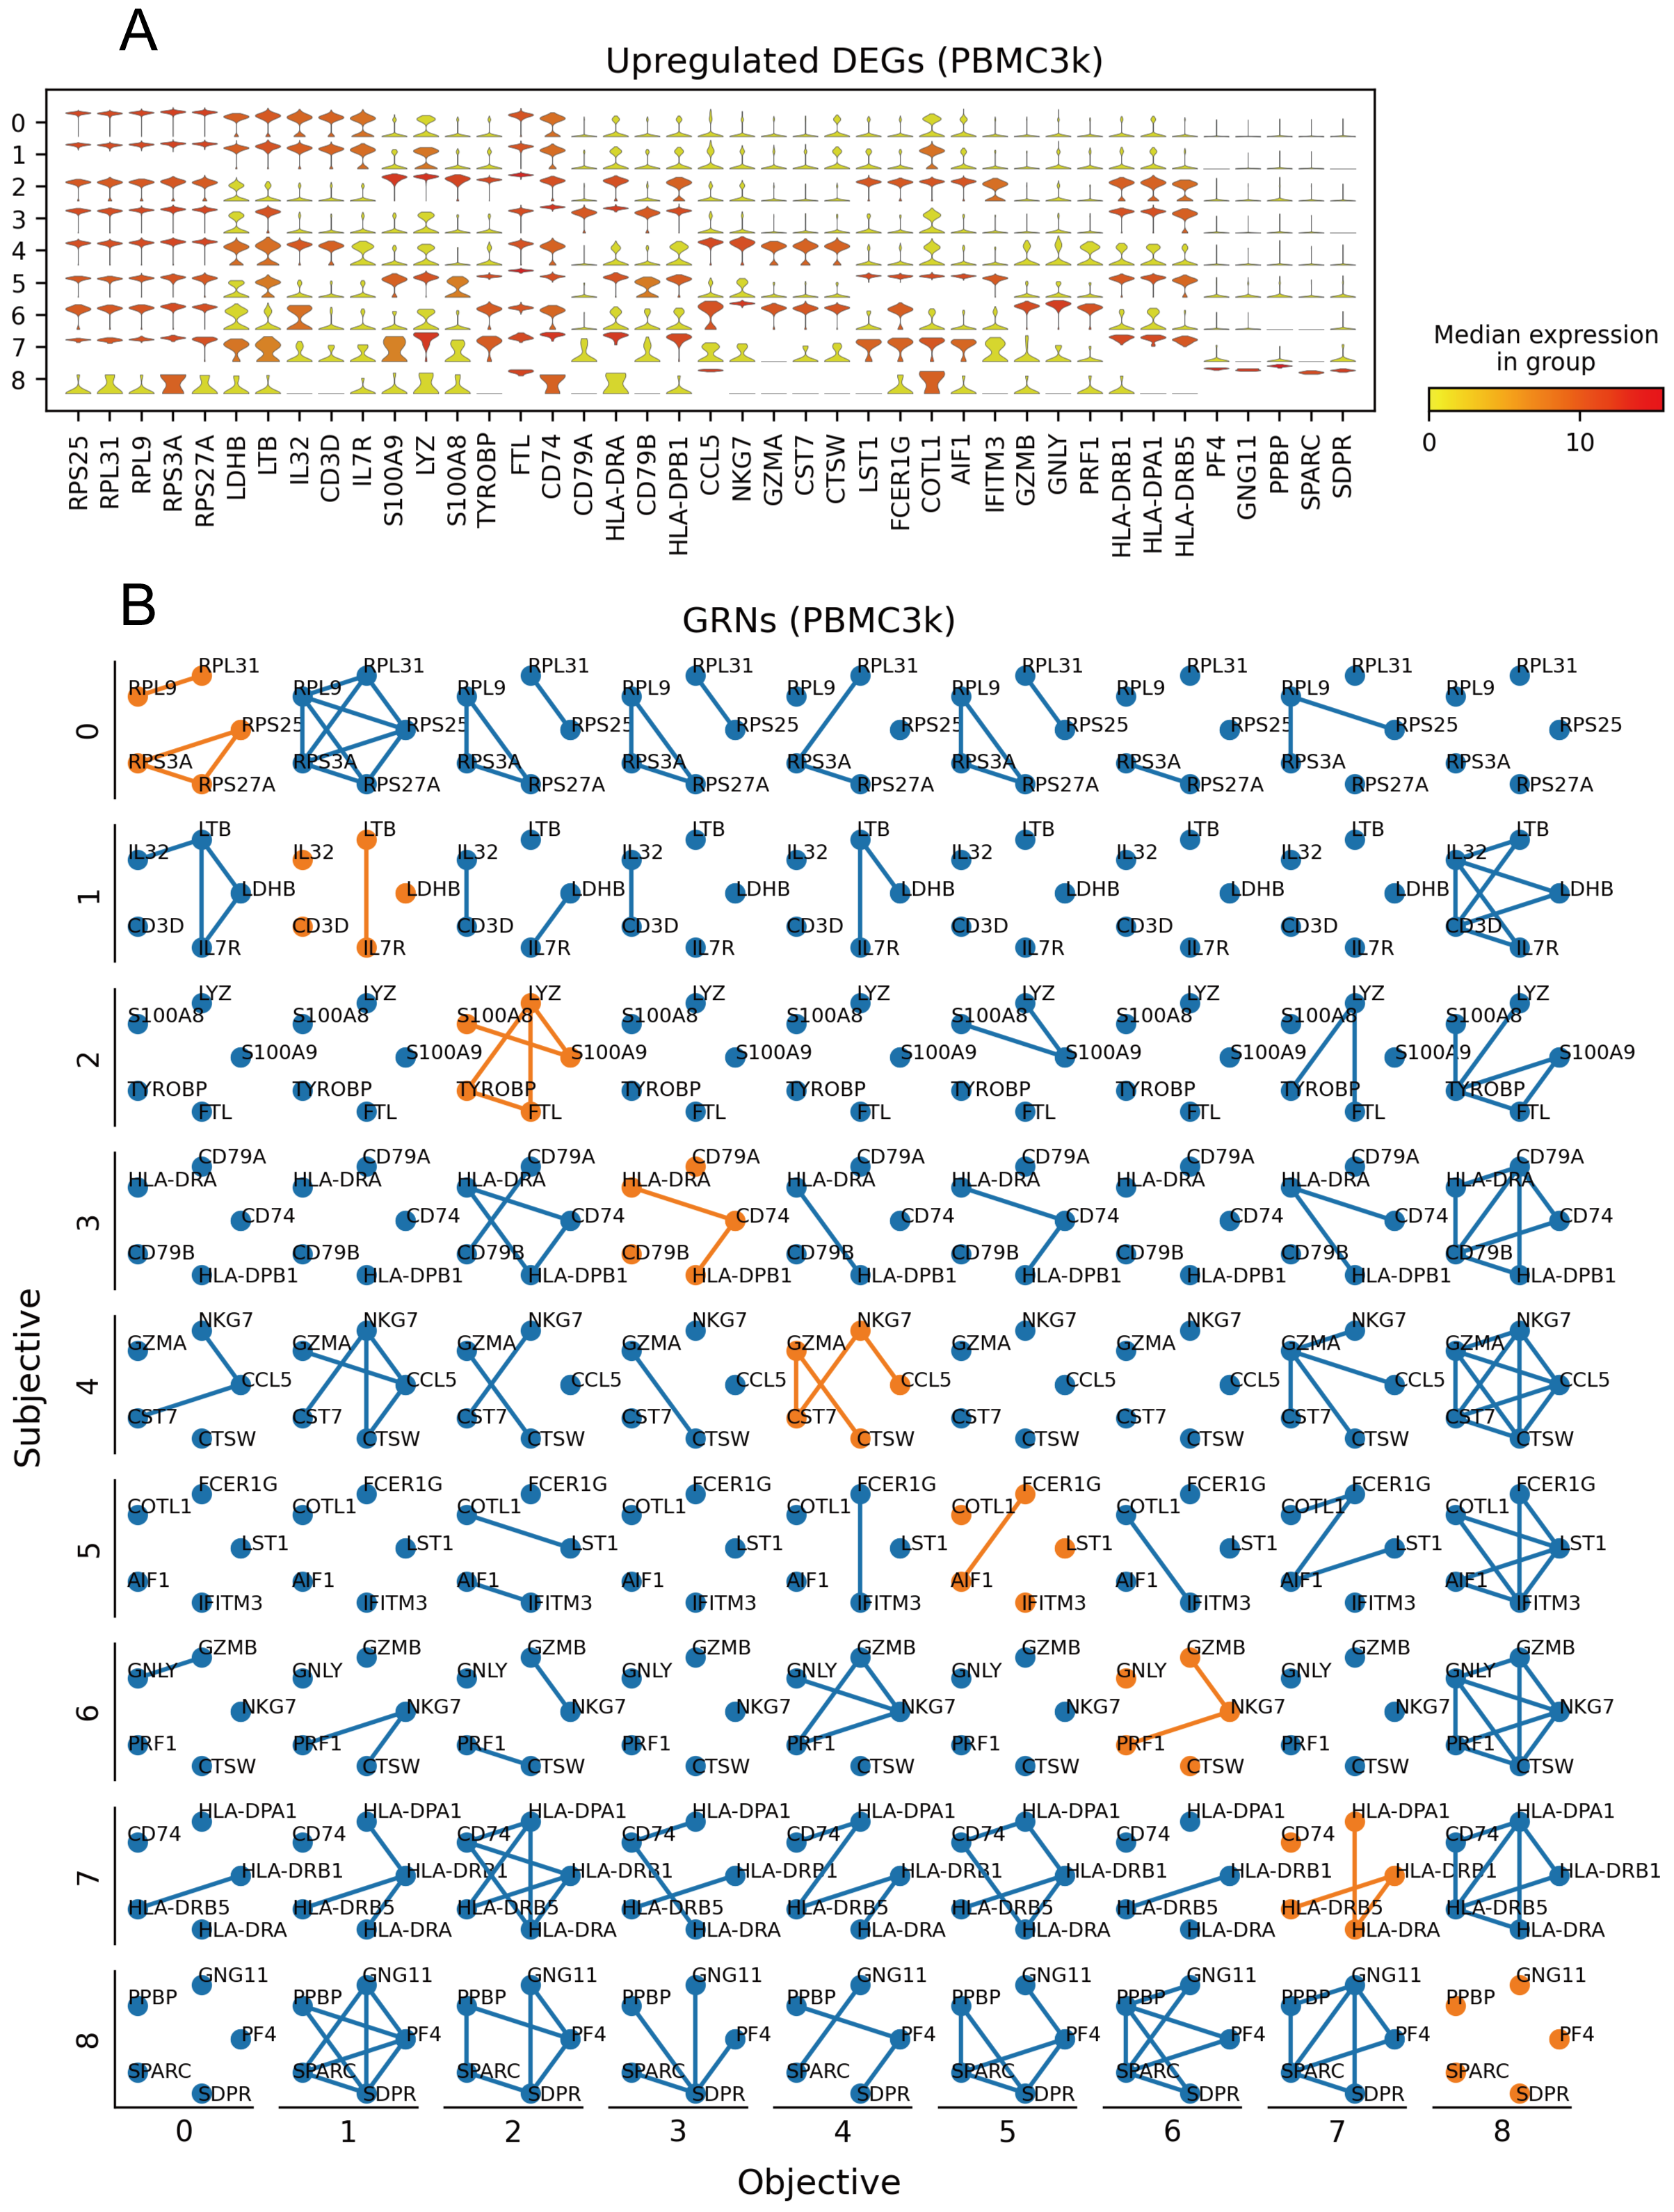
\includegraphics[scale=0.75]{./figs/exported/figure_s4.png}
  \caption{The top 5 DEGs and the GRNs of the clusters in PBMC3k}
  \legend{
    \textbf{A}: Violin plot of DEGs of the clusters (top 5 for each)
    \textbf{B}: GRNs of the clusters. GRNs in a row share the same set of genes
    (DEGs of the subjective clusters) selected for the vertex sets
  }
  \label{fig_s4}
\end{figure}
\begin{figure}[htb]
  \centering
  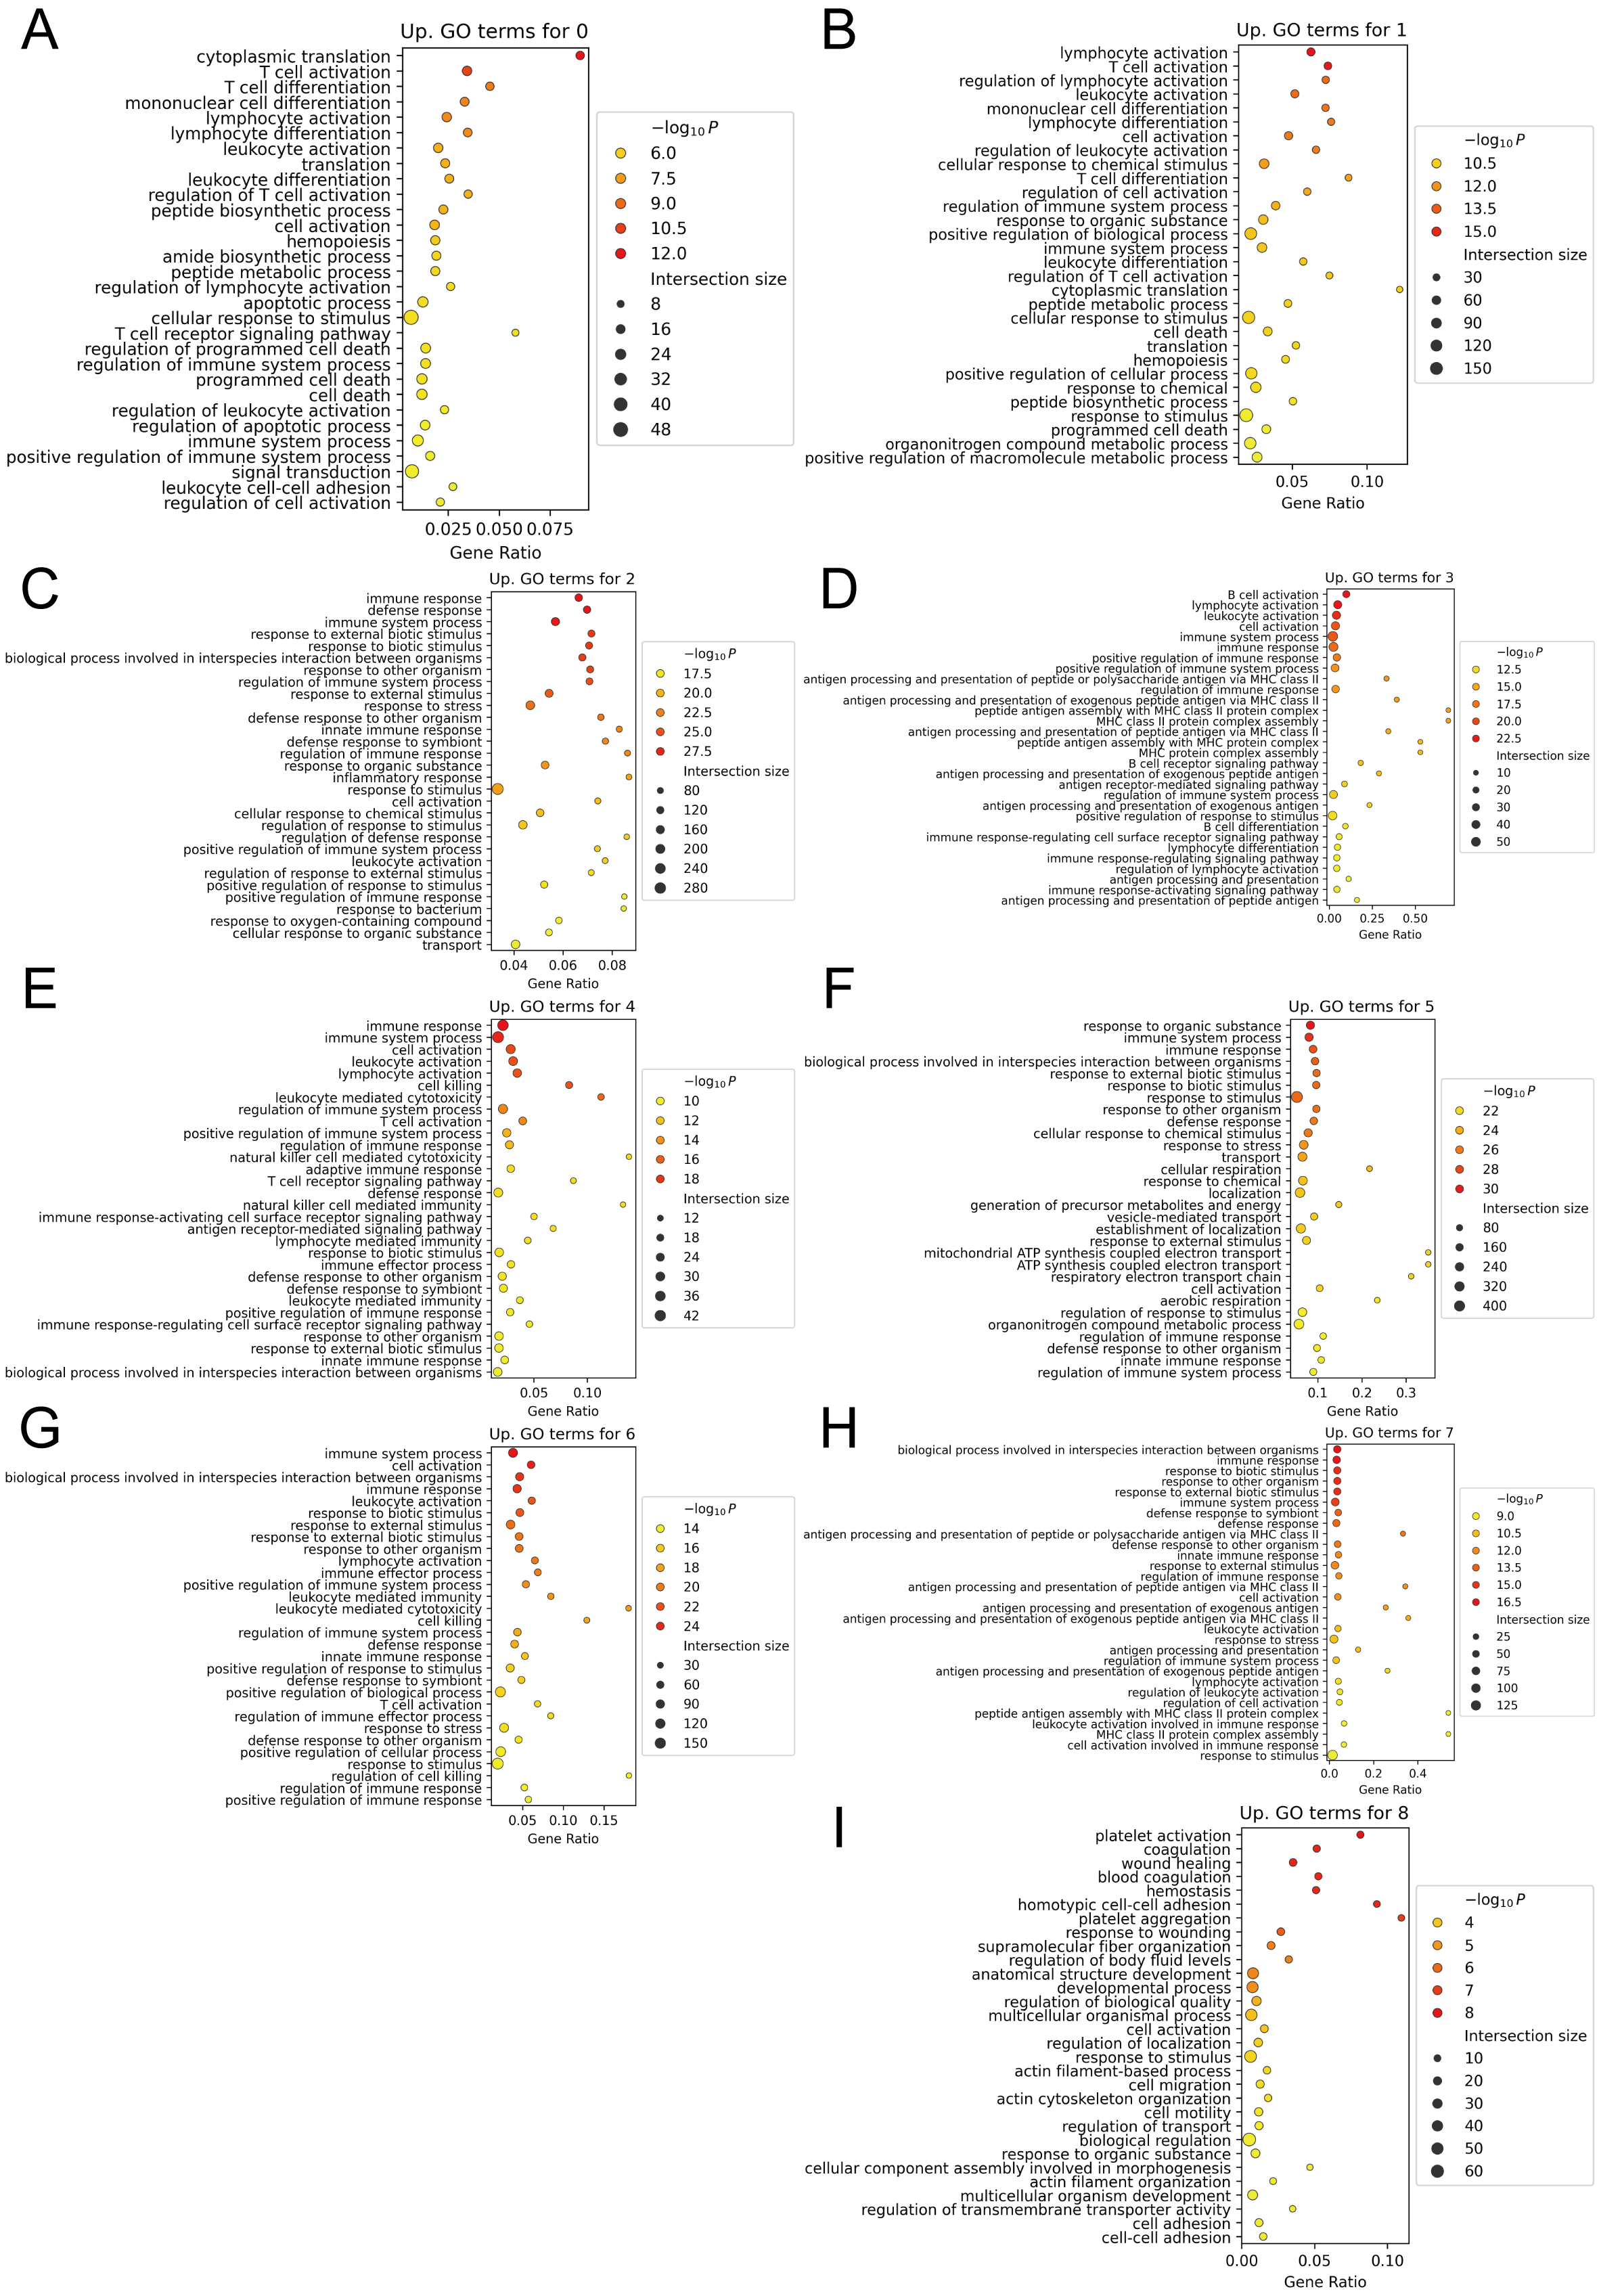
\includegraphics[scale=0.7]{./figs/exported/figure_s5.png}
  \caption{The top 30 upregulated GO terms of the clusters in PBMC3k}
  \legend{
    \textbf{A-I}: The top 30 GO terms for cluster 0$\sim$8 respectively
  }
  \label{fig_s5}
\end{figure}
\begin{figure}[htb]
  \centering
  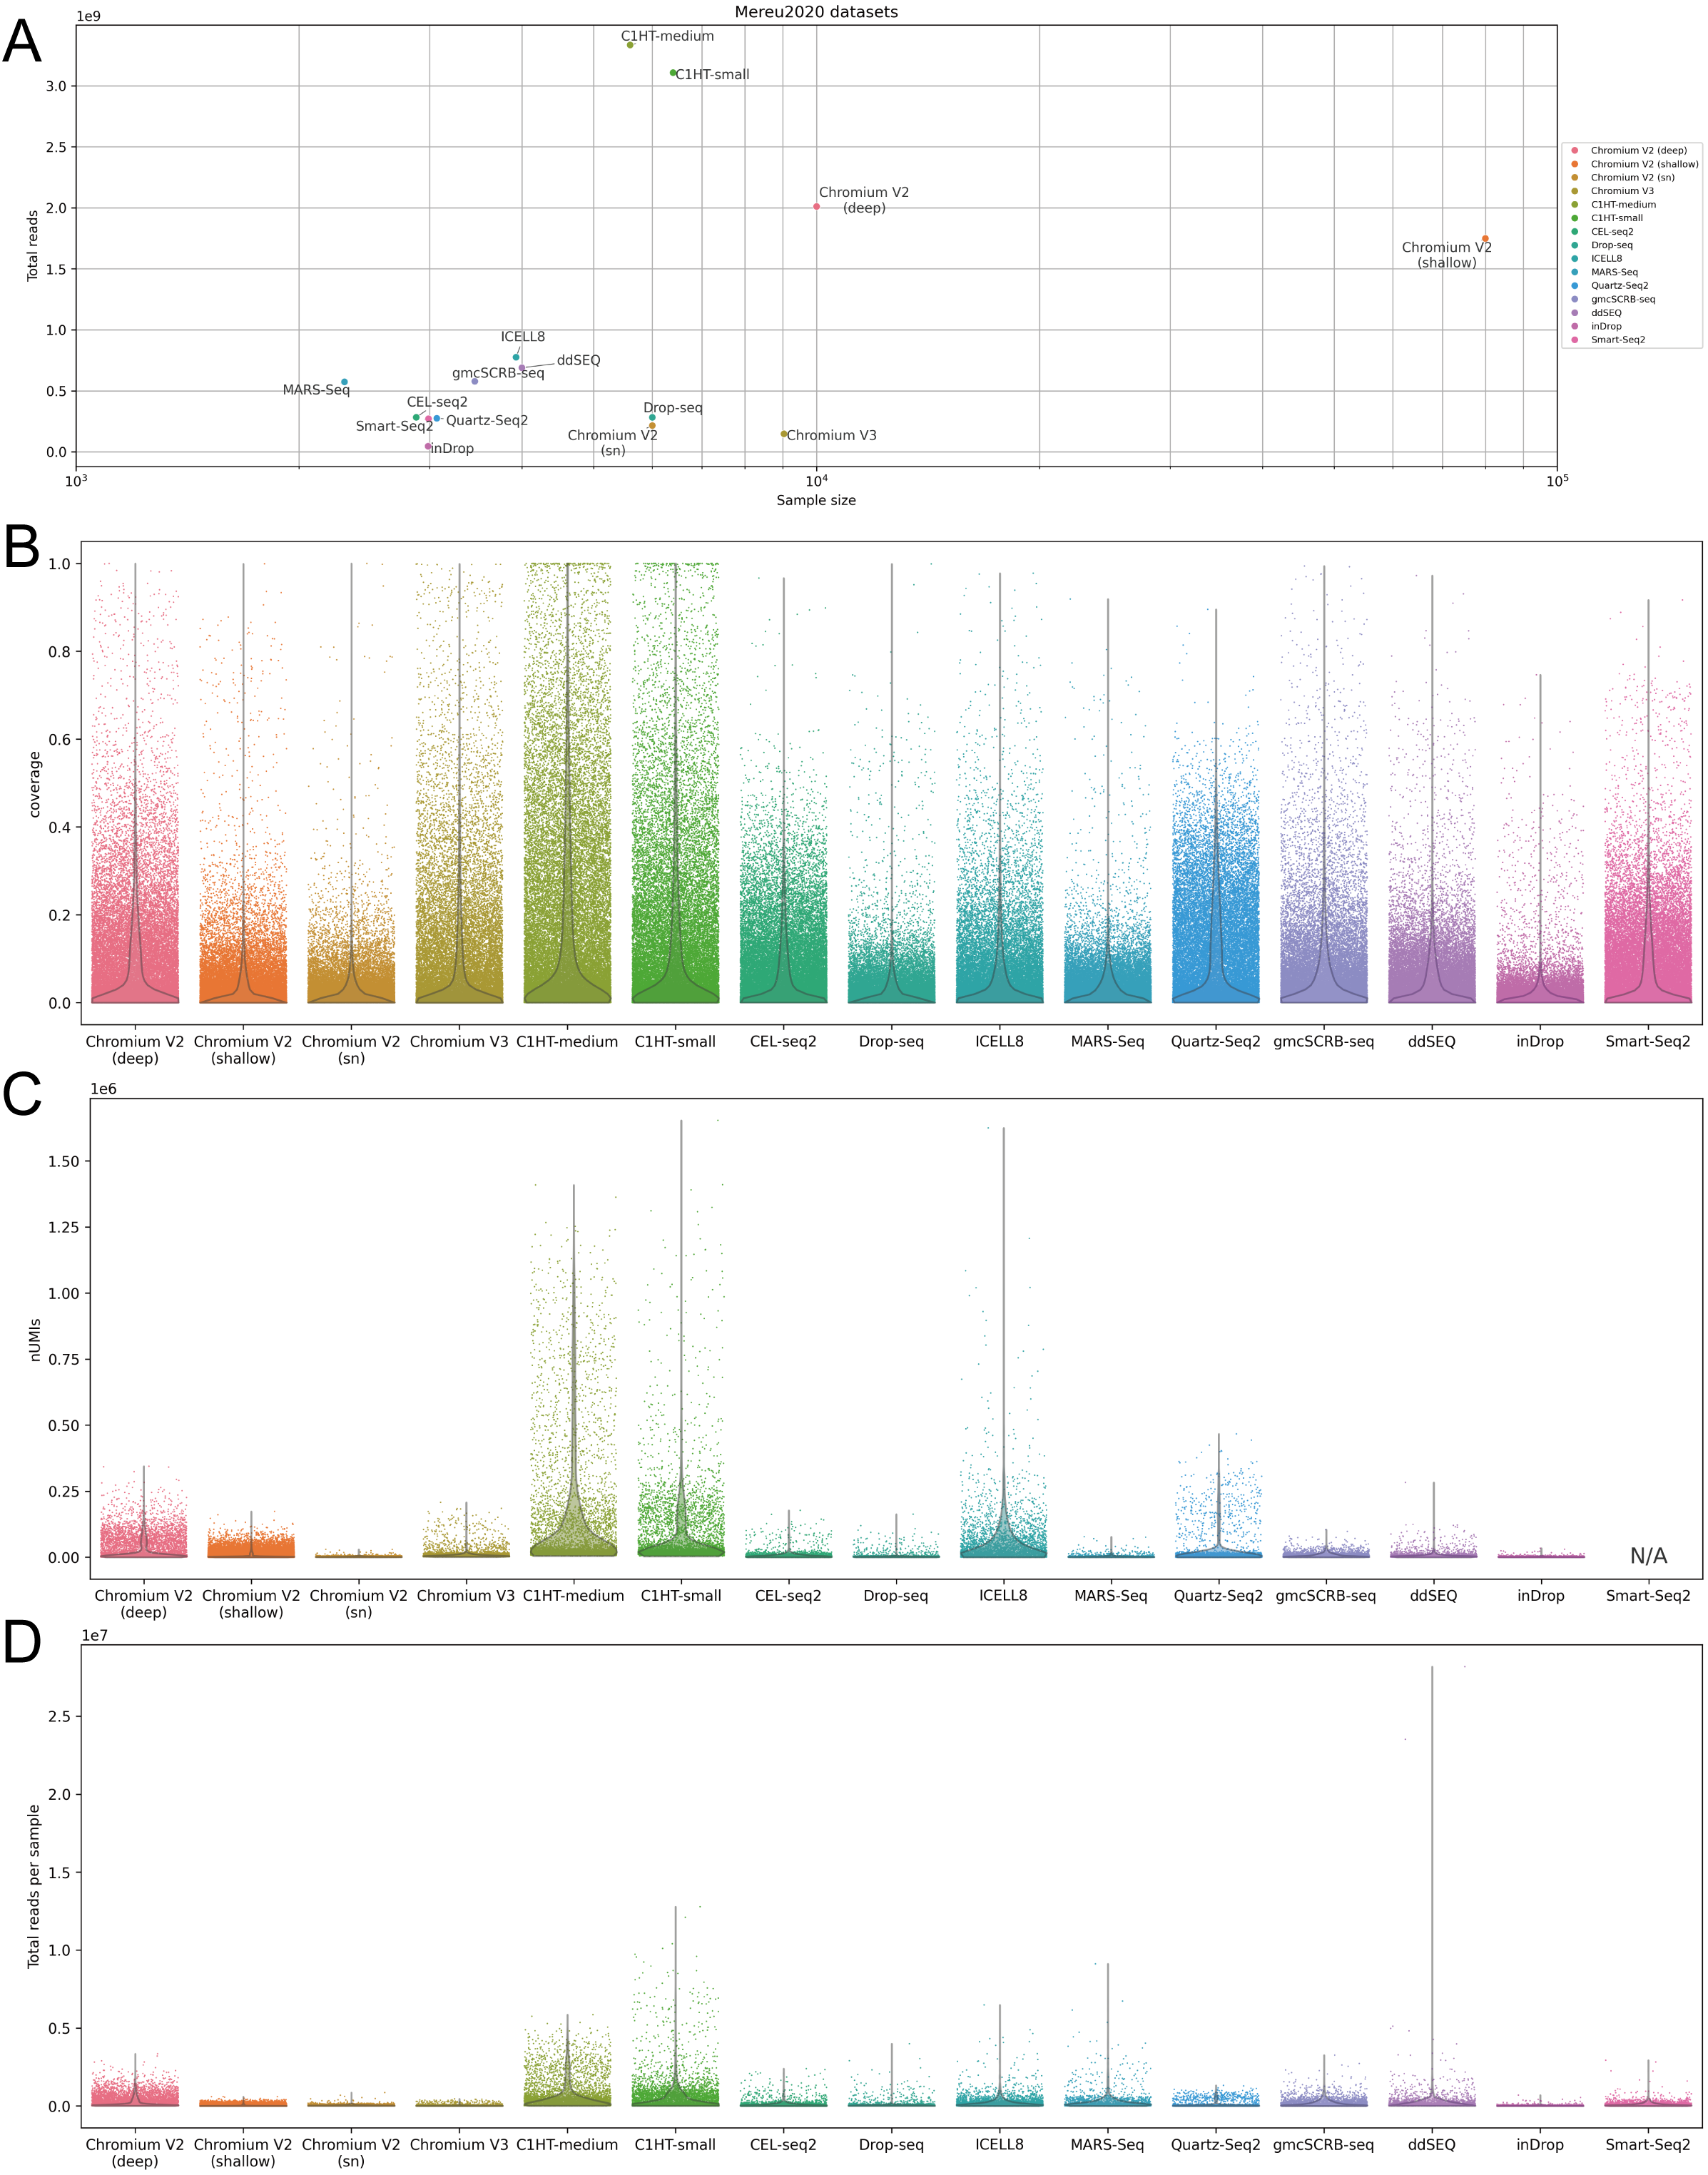
\includegraphics[scale=0.7]{./figs/exported/mereu2020.png}
  \caption{Mereu2020 datasets}
  \legend{
    \textbf{A}: A scatter plot regarding the sample sizes and the total reads of the superfamilies in Mereu2020.
    \textbf{B}: Coverages in the superfamilies in Mereu2020. The dots of the strip plots refer the coverage values of genes in each dataset.
    \textbf{C}: Numbers of UMIs (nUMIs) in Mereu2020. As SmartSeq2 is not UMI-based, data were not available.
    \textbf{D}: Total reads per sample in Mereu2020 datasets.
  }
  \label{fig_s6}
\end{figure}
\begin{figure}[htb]
  \centering
  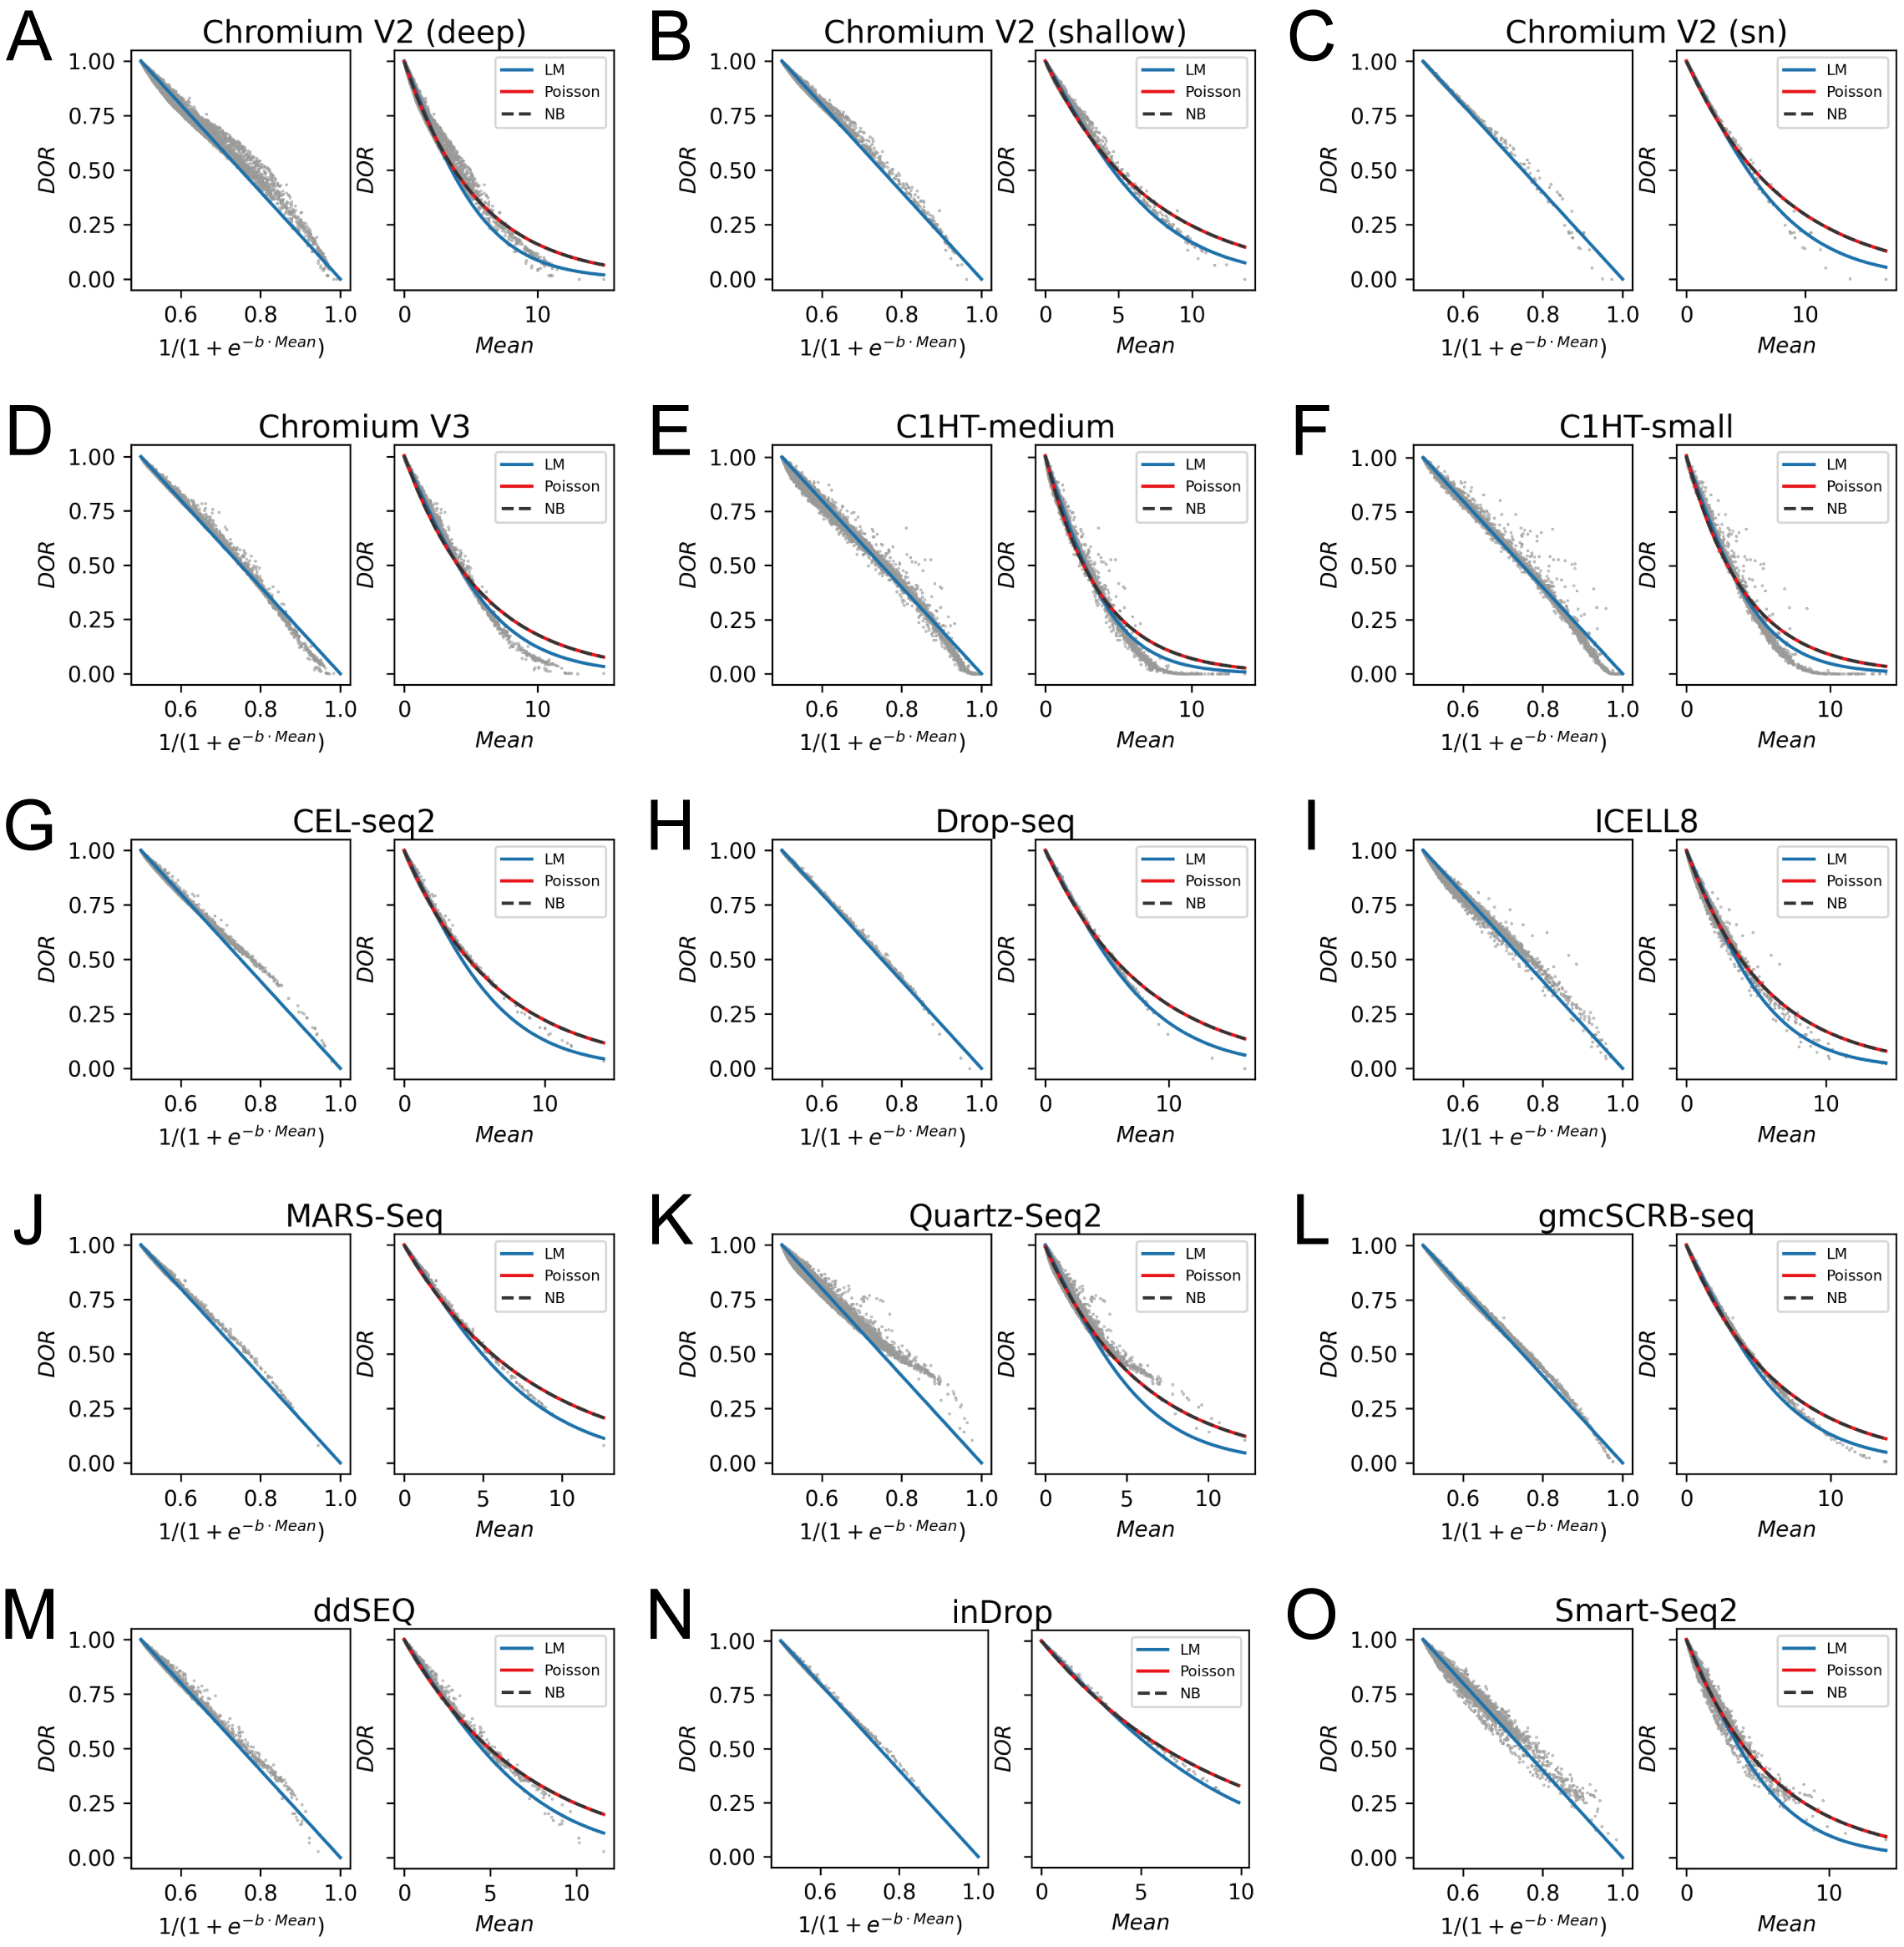
\includegraphics[scale=0.7]{./figs/exported/mereu2020_lm.png}
  \caption{Regression models of DOR in Mereu2020 datasets}
  \legend{
    \textbf{A-O}: A scatter plot regarding the sample sizes and the total reads of the superfamilies in Mereu2020.
  }
  \label{fig_s7}
\end{figure}
\begin{figure}[htb]
  \centering
  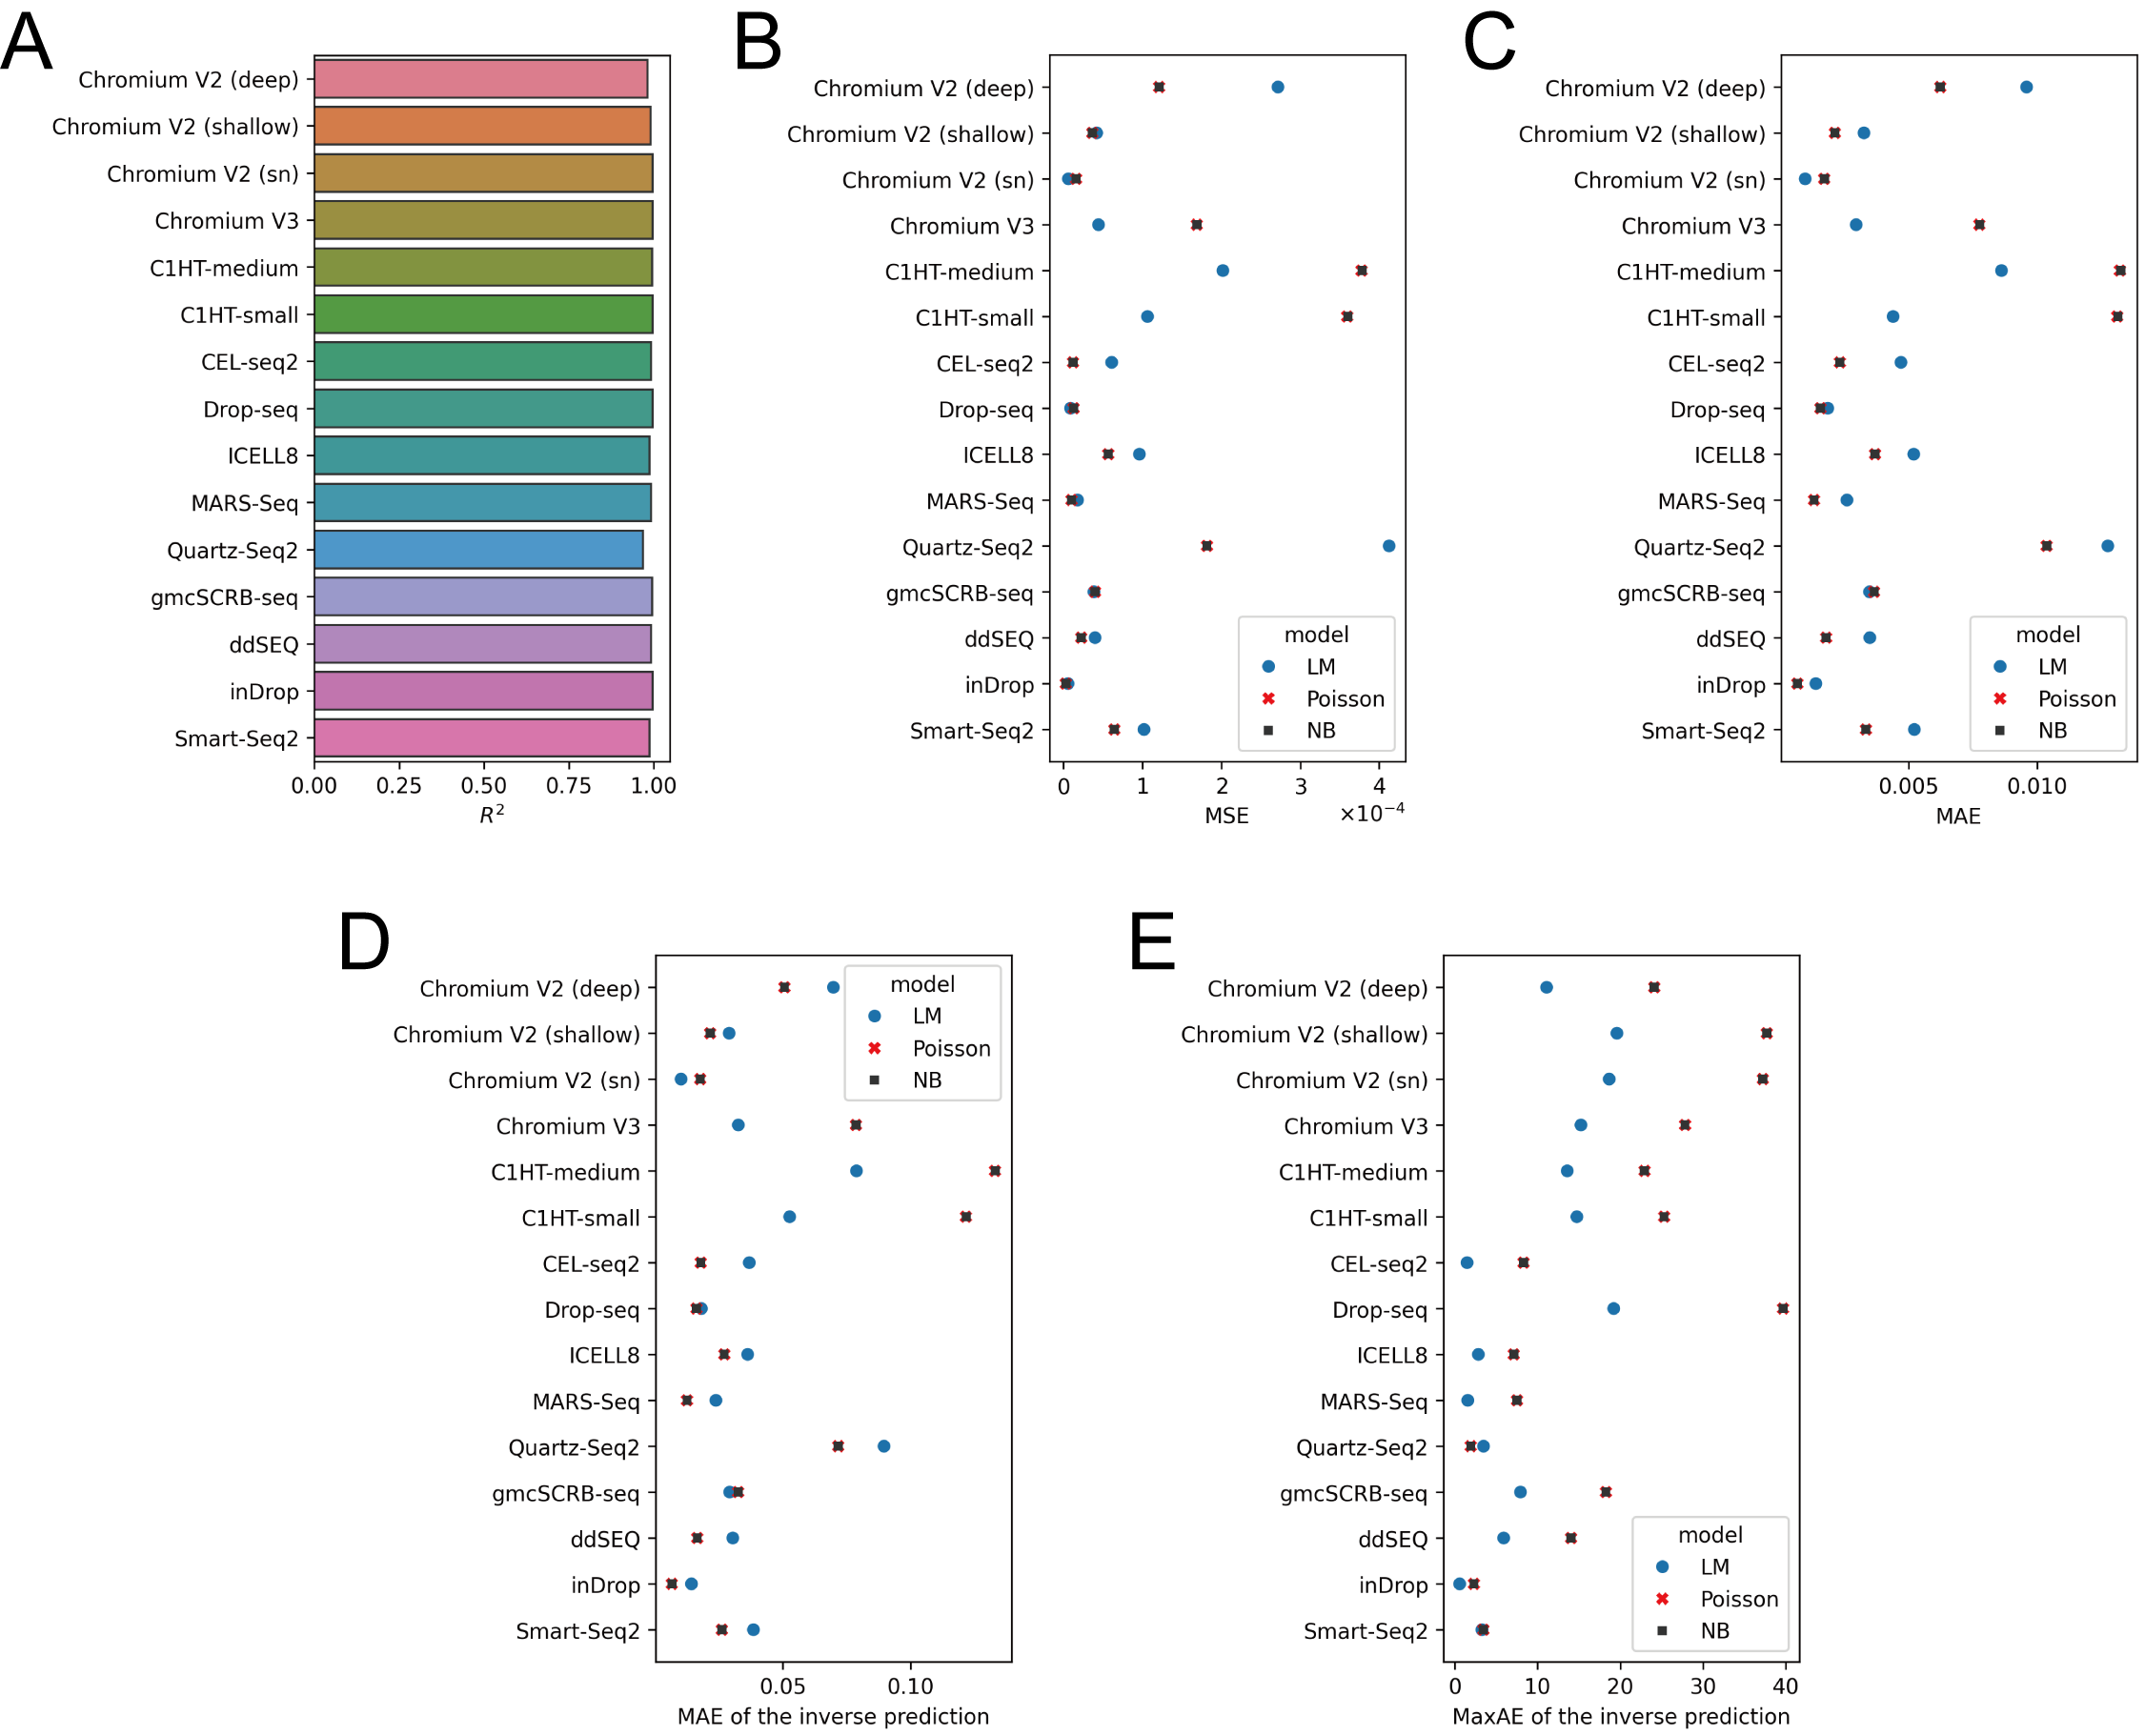
\includegraphics[scale=0.7]{./figs/exported/mereu2020_metrics.png}
  \caption{Performance metrices for regression models of DOR in Mereu2020 datasets}
  \legend{
    \textbf{A}: The coefficients of determination ($R^2$) of logistic-transformed mean expression values to the linear calibration curve of DOR.
    \textbf{B}: Performance comparison of LM, Poisson, and NB with MSE values.
    \textbf{C}: Performance comparison of LM, Poisson, and NB with MAE values.
    \textbf{D}: Performance comparison of the inverse predictions of LM, Poisson, and NB with MAE values.
    \textbf{E}: Performance comparison of the inverse predictions of LM, Poisson, and NB with MaxAE values.
  }
  \label{fig_s8}
\end{figure}

\end{document}
